\section{Methodology}
\label{method}
Our goal was to run the HouseDiffusion architecture \cite{HouseDiffusion} on
ResPlan rather than RPLAN. We keep its transformer backbone, attention design, and
diffusion process; the only change to the network follows from widening the input
representation. The work therefore centred on two problems: building a clean and
reproducible training pipeline, and reshaping the more complex ResPlan plans into
the fixed-width representation the model expects without discarding most of the
dataset.
Table~\ref{tab:model_card} gives the consolidated specification of the final
model.

\begin{table}[t]
  \centering
  \small
  \setlength{\tabcolsep}{4pt}
  \renewcommand{\arraystretch}{1.15}
  \begin{tabular}{@{}>{\bfseries}l p{0.60\linewidth}@{}}
    \toprule
    Model Name & HouseDiffusion-ResPlan \\
    Version & 1.0 (Fall 2025) \\
    Architecture & Transformer denoising diffusion model; $512$-dim, $4$ heads,
      per-layer component, relational, and global attention; continuous
      corner-coordinate denoising \\
    Framework & PyTorch $\geq 2.1$ with PyTorch Lightning \\
    Training Data & ResPlan ($\sim$17k floorplans); $\sim$93\% retained at the
      192-point budget \\
    Input Format & Per-vertex $158$-dim feature (\texttt{c158p192}): 2D
      coordinates, $25$-way room type, $64$ corner index, $64$ room index; up
      to $192$ points per plan, coordinates in $[-1,1]$ \\
    Output & Vector floorplan: polygonal room and door loops as 2D corner
      coordinates \\
    Hyperparameters & AdamW (lr $3\times10^{-4}$, weight decay $0.05$), batch
      size $64$, fp32; $1000$-step cosine diffusion; EMA $0.9999$; $2000$-step
      warmup; up to $250$k steps \\
    Intended Use & Research prototype generating synthetic 2D floorplans as test
      data for Milestone Systems (non-production) \\
    Limitations & Plans over $192$ vertices dropped ($\sim$7\% of ResPlan);
      sensitive to fp16 overflow (needs an fp32 fallback); one-hot constraints
      only, no GNN or guided sampling; limited by ResPlan scale and its
      room-type vocabulary \\
    \bottomrule
  \end{tabular}
  \caption{Model card for HouseDiffusion-ResPlan (stable fp32 configuration).}
  \label{tab:model_card}
\end{table}

\subsection{Training pipeline}
We reimplemented the training loop on top of PyTorch Lightning \cite{lightning}. This separates
the optimisation logic from the data and model code and gives us logging,
checkpointing, and multi-GPU support without extra bookkeeping. Each step samples
a diffusion timestep, computes the denoising loss, and updates an exponential
moving average of the weights. We optimise with AdamW under a linear warmup
followed by a stepwise learning-rate decay; the exact hyperparameters of the
reported model are listed in Table~\ref{tab:model_card}. Validation runs on a
held-out split at a fixed global-step
interval rather than once per epoch, which keeps the validation signal comparable
across runs of different epoch length. We keep the diffusion process from the
original work \cite{HouseDiffusion, DDPM}: $1000$ timesteps with a cosine noise
schedule, a $512$-channel transformer, and continuous denoising of the corner
coordinates. Training is configured for a single NVIDIA L40S GPU on the DTU HPC
cluster, with a 24-hour wall-clock budget.

\subsection{Adapting the representation to ResPlan}
HouseDiffusion encodes a floorplan as a fixed-width array, one row per polygon
vertex, zero-padded to a maximum number of points, with any plan exceeding that
limit discarded. The original format was tuned to the comparatively simple RPLAN
apartments; ResPlan plans have more rooms and more detailed outlines, so we
widened every field (Table~\ref{tab:repr}). The larger point budget keeps about
$93\%$ of ResPlan, against roughly $57\%$ at a $128$-point budget. The full row is
a $158$-dimensional per-vertex feature (the \texttt{c158p192} schema): the 2D
coordinates, a one-hot room type, one-hot corner and room indices, and the
auxiliary fields used by the model.

\begin{table}[t]
  \centering
  \small
  \setlength{\tabcolsep}{6pt}
  \renewcommand{\arraystretch}{1.15}
  \begin{tabular}{@{}l c c@{}}
    \toprule
    & RPLAN (orig.) & ResPlan (ours) \\
    \midrule
    Max points per plan   & $100$ & $192$ \\
    Corner-index width    & $32$  & $64$  \\
    Room-index width      & $32$  & $64$  \\
    Room-type one-hot     & $25$  & $25$  \\
    Conditioning channels & $89$  & $153$ \\
    \bottomrule
  \end{tabular}
  \caption{Representation widths in the original HouseDiffusion (RPLAN) versus our
  ResPlan port. Only the point budget and index widths change; the conditioning
  size follows as room-type $+$ corner $+$ room ($25+64+64=153$).}
  \label{tab:repr}
\end{table}

Doubling the corner and room index widths grows the conditioning vector from $89$
to $153$ channels, which enlarges the model's first conditioning layer
(\texttt{Linear}$(89,512)\rightarrow$\texttt{Linear}$(153,512)$). The released
RPLAN weights are therefore no longer compatible and we train from scratch. The
wider point budget also raises the training cost: the transformer's self-attention
is quadratic in the number of points, so moving from $100$ to $192$ points
increases the per-layer attention cost by about $3.7\times$.

\subsection{Polygon simplification}
Even after widening the format, a small number of ResPlan rooms have very
detailed outlines with many near-collinear vertices that add little structure but
consume the point budget and make the geometry harder to denoise. We added a
simplification step that reduces a room outline to at most the corner limit
before encoding. It applies Shapely's topology-preserving \texttt{simplify} with
an exponentially increasing tolerance until the outline meets the corner budget,
and leaves rooms that are already within the limit untouched. This keeps more
plans inside the representation and gives the model cleaner targets to learn from.

\begin{figure*}[t]
  \centering
  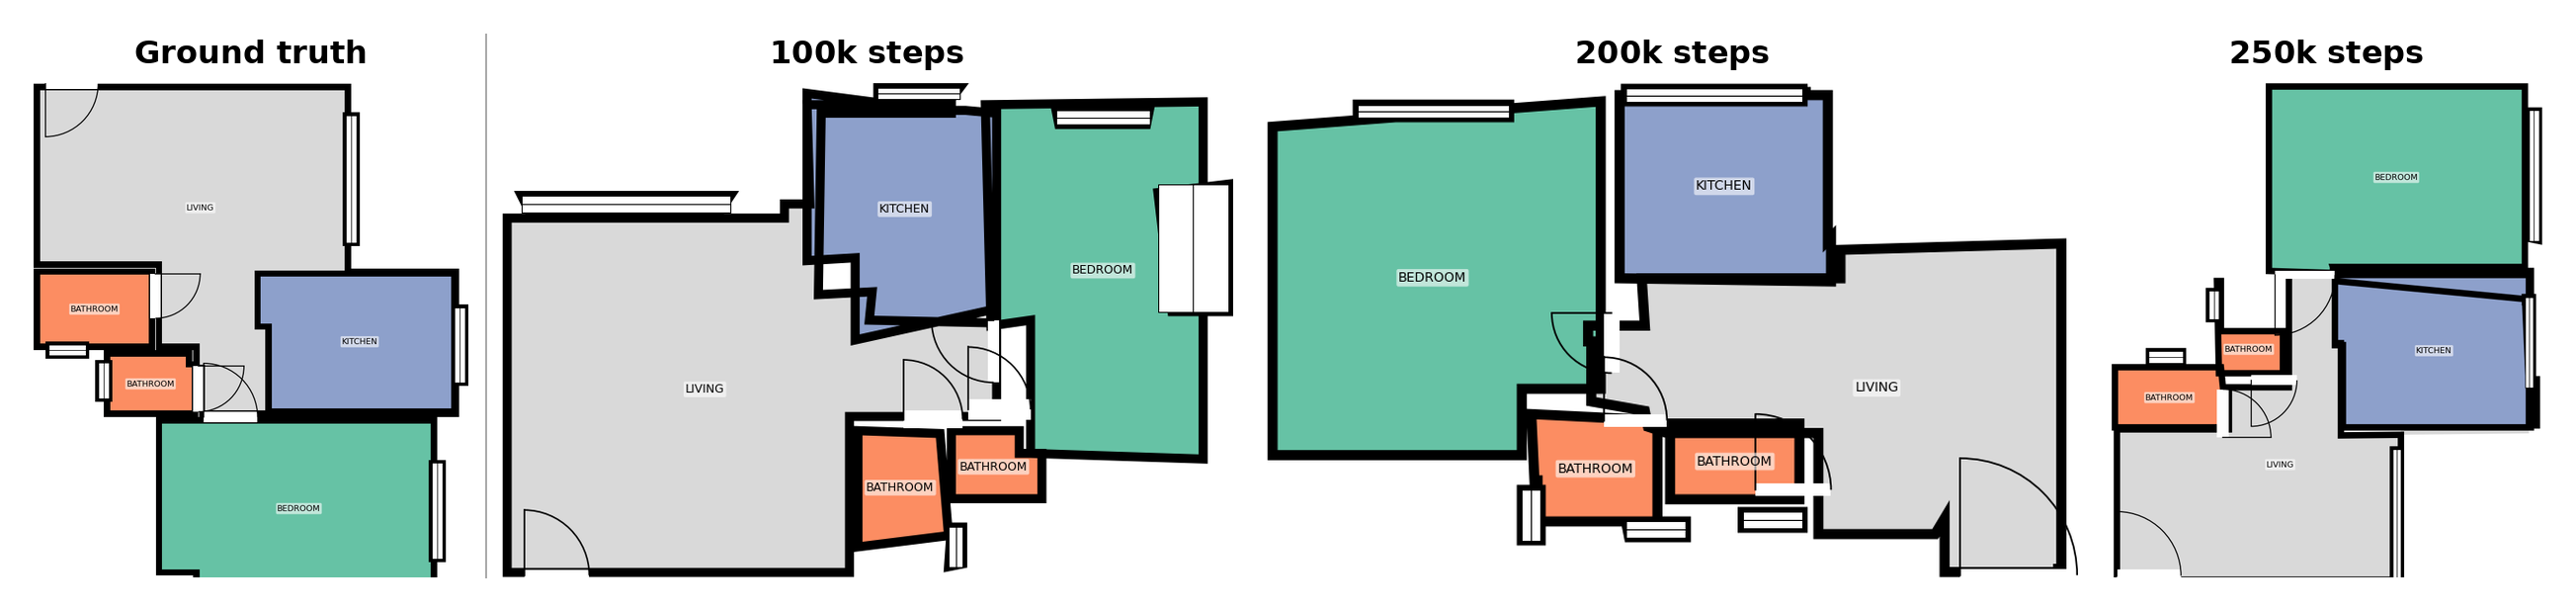
\includegraphics[width=\linewidth]{figures/progression.png}
  \caption{Generation quality over training for one held-out plan: the ground
  truth (left) and samples from the model at $100$k, $200$k, and $250$k steps. The
  conditioning rooms and their adjacencies are already recovered by $100$k steps;
  later checkpoints mainly refine the geometry, with room outlines tiling more
  cleanly and fewer overlaps.}
  \label{fig:training_progress}
\end{figure*}
